\ifbilingual\begin{figure}[tb]\else\begin{figure}[t]\fi
\centering
\ifbilingual
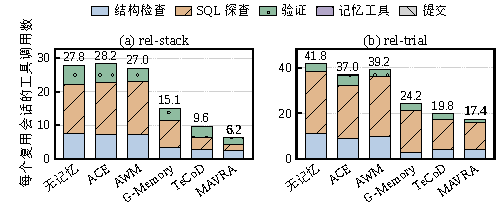
\includegraphics[width=\linewidth]{figures/reuse-work-zh}
\else
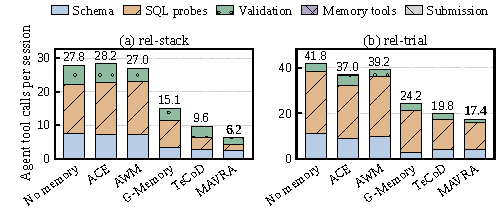
\includegraphics[width=\linewidth]{figures/reuse-work}
\fi
\caption{\bt{Agent-issued tool calls per reuse session at cutoffs 2--3 (six sessions per method and database, failures included).}{截点 2--3 每个复用会话的智能体工具调用数（每种方法、每个数据库六个会话，含失败）。}}
\label{fig:reuse-work}
\Description{Two side-by-side panels, one per database, compare all five methods. Stacked bars distinguish schema inspection, SQL probes, validation, memory tools, and submission with colors and hatching. The y-axis counts agent-issued tool calls per reuse session and starts at zero.}
\end{figure}
